Discuss the simplified OpenMC model for preliminary results (maybe include flow diagram).

\begin{figure}[H]
    \centering
    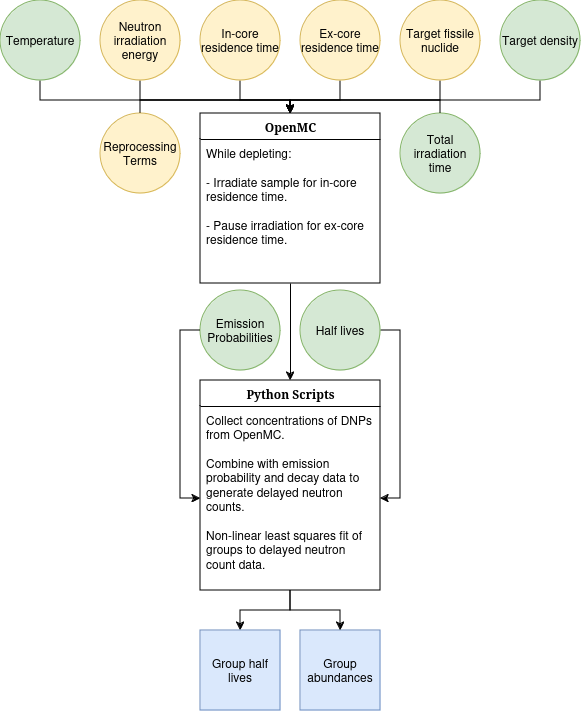
\includegraphics[width=0.5\linewidth]{images/simplified-model.png}
    \caption{Flow diagram of simplified model used to generate flow-inclusive precursor group fit parameters.}
    \label{fig:simplified-model}
\end{figure}

3 gram spherical sample

fixed source problem

OpenMC provided chain files (pwr for thermal energy and sfr for fast energy)

Thermal energy uses 0.0253 eV, fast uses 0.7 MeV.

Using N(t) rather than exponential decay in order to capture decays (include comparison figure)

delayed neutron yield calculations: OpenMC only, concentrations integral

Weighted least squares using adjusted counts as weights